\documentclass[]{article}

\usepackage{amsmath}
\usepackage{graphicx}
\usepackage{float}
\usepackage{multicol}
\usepackage{fancyhdr}
\fancyhead[L, CO] {}
\fancyhead[C, CO] {PartDiff - Résumé 2021}
\fancyhead[R, CO] {}
\usepackage[margin=1.5cm,landscape,includehead]{geometry}
\pagestyle{fancy}
\usepackage{mathtools} % for '\splitdfrac' macro
\usepackage[dvipsnames]{xcolor}


\begin{document}
\begin{multicols}{3}
\section{Intégration}
\subsection{Intégration par partie}
$$\int_{a}^{b}u'v=uv\Big|_{a}^{b}-\int_{a}^{b}uv'$$
\section{Différences finies}
\subsection{Différences finies progressives}
\subsubsection{$f'(x)$}
\begin{figure}[H]
\centering
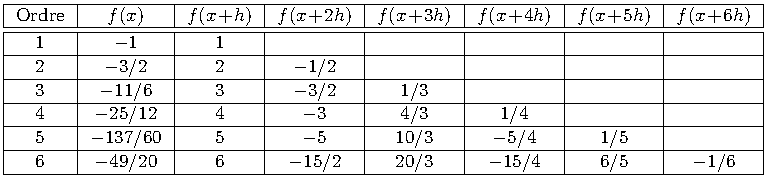
\includegraphics[width=\columnwidth,page=1]{diff_finies_tableaux.pdf}
\end{figure}
$\textcolor{ForestGreen}{n=2}$
$$f\textcolor{OrangeRed}{'}(x)=\frac{-\frac{3}{2}f(x)+2f(x+h)-\frac{1}{2}f(x+2h)}{\textcolor{OrangeRed}{h}}+\mathcal{O}(h^{\textcolor{ForestGreen}{2}})$$
\subsubsection{$f''(x)$}
\begin{figure}[H]
\centering
\includegraphics[width=\columnwidth,page=2]{diff_finies_tableaux.pdf}
\end{figure}
$\textcolor{ForestGreen}{n=3}$
$$f\textcolor{OrangeRed}{''}\left(x\right)=\frac{\splitdfrac{\splitdfrac{\frac{35}{12}f\left(x\right)}{-\frac{26}{3}f\left(x+h\right)+\frac{19}{2}f\left(x+2h\right)}}{-\frac{14}{3}f\left(x+3h\right)+\frac{11}{12}f\left(x+4h\right)}}{h^{\textcolor{OrangeRed}{2}}}+\mathcal{O}(h^{\textcolor{ForestGreen}{3}})$$
\subsubsection{$f'''(x)$}
\begin{figure}[H]
\centering
\includegraphics[width=\columnwidth,page=3]{diff_finies_tableaux.pdf}
\end{figure}
$\textcolor{ForestGreen}{n=1}$
$$f\textcolor{OrangeRed}{'''}\left(x\right)=\frac{\splitdfrac{-f\left(x\right)+3f\left(x+h\right)}{-3f\left(x+2h\right)+f\left(x+3h\right)}}{h^{\textcolor{OrangeRed}{3}}}+\mathcal{O}(h^{\textcolor{ForestGreen}{1}})$$
\subsection{Différences finies rétrogrades}
\begin{enumerate}
\item Remplacer $x+kh$ par $x-kh$
\item Si dérivée paire : Pas de changement de coefficient
\item Si dérivée impaire : Changement du signe
\end{enumerate}
\subsection{Différences finies centrées}
\subsubsection{$f'(x)$}
\begin{figure}[H]
\centering
\includegraphics[width=\columnwidth,page=5]{diff_finies_tableaux.pdf}
\end{figure}
$\textcolor{ForestGreen}{n=2}$
$$f\textcolor{OrangeRed}{'}(x)=\frac{-\frac{1}{2}f(x-h)+\frac{1}{2}f(x+h)}{h^{\textcolor{OrangeRed}{1}}}+\mathcal{O}(h^{\textcolor{ForestGreen}{2}})$$
\subsubsection{$f''(x)$}
\begin{figure}[H]
\centering
\includegraphics[width=\columnwidth,page=6]{diff_finies_tableaux.pdf}
\end{figure}
$\textcolor{ForestGreen}{n=2}$
$$f\textcolor{OrangeRed}{''}(x)=\frac{f(x-h)-2f(x)+f(x+h)}{h^{\textcolor{OrangeRed}{2}}}+\mathcal{O}(h^{\textcolor{ForestGreen}{2}})$$
\subsubsection{$f'''(x)$}
\begin{figure}[H]
\centering
\includegraphics[width=\columnwidth,page=7]{diff_finies_tableaux.pdf}
\end{figure}
$\textcolor{ForestGreen}{n=2}$
$$f\textcolor{OrangeRed}{'''}(x)=\frac{\splitdfrac{-\frac{1}{2}f(x-2h)+f(x-h)}{-f(x+h)+\frac{1}{2}f(x+2h)}}{h^{\textcolor{OrangeRed}{3}}}+\mathcal{O}(h^{\textcolor{ForestGreen}{2}})$$



\end{multicols}
\end{document}